\documentclass[10pt,twocolumn]{article}

\usepackage[a4paper,margin=1.8cm]{geometry}
\usepackage{amsmath,amssymb}
\usepackage{booktabs}
\usepackage{graphicx}
\usepackage{xcolor}
\usepackage{hyperref}
\usepackage{enumitem}
\usepackage{fancyhdr}
\usepackage{caption}
\usepackage{abstract}

\hypersetup{colorlinks=true, linkcolor=blue!50!black, citecolor=blue!50!black, urlcolor=blue!50!black}
\newcommand{\ohm}{\ensuremath{\Omega}}
\newcommand{\degC}{\ensuremath{^{\circ}\mathrm{C}}}
\setlength{\abstitleskip}{-1em}
\setlength{\absleftindent}{0pt}
\setlength{\absrightindent}{0pt}

\pagestyle{fancy}
\setlength{\headheight}{14pt}
\fancyhf{}
\rhead{\footnotesize EPC2361 Half-Bridge Building Block}
\lhead{\footnotesize Design \& Loss Analysis}
\cfoot{\thepage}

% Auto-generated by scripts/make_report_values.py -- do not edit by hand.
\newcommand{\NVAL}{4}
\newcommand{\RGONVAL}{0.5}
\newcommand{\RGOFFVAL}{2.7}
\newcommand{\FSWVAL}{99.3}
\newcommand{\PTOTALVAL}{27.12}
\newcommand{\PBUDGETVAL}{31.41}
\newcommand{\PCTVAL}{86}
\newcommand{\TJVAL}{62.4}
\newcommand{\MARGINVAL}{62.6}
\newcommand{\OVSVAL}{14.8}


\title{\vspace{-1em}\textbf{\large Design of a GaN Half-Bridge Building Block for a Stacked\\
Poly-Phase Bridge: EPC2361, 75\,V / 6.25\,kW}\vspace{-0.5em}}
\author{\footnotesize SPB Building-Block Design Toolkit \\[-0.3em] \footnotesize \today}
\date{}

\begin{document}
\maketitle

\begin{abstract}
\noindent This paper reports the electrical and thermal design of one half-bridge
building block of a stacked poly-phase bridge, using the EPC2361 100\,V eGaN HEMT. Gate
turn-on and turn-off resistance are optimized independently against a full 120-point
LTSpice double-pulse characterization spanning device current, gate resistance, and
power-loop inductance, run against the vendor's own SPICE model. The recommended point
--- \textbf{N=\NVAL{} devices in parallel per switch position, $R_{g,on}$=\RGONVAL\,\ohm,
$R_{g,off}$=\RGOFFVAL\,\ohm, $f_{sw}\approx$\FSWVAL\,kHz} --- meets a 99.5\% full-load
efficiency target and a 125\,\degC{} junction-temperature ceiling with margin, using
thermal and power-loop parameters grounded in three independent published GaN
half-bridge designs rather than assumed values.
\end{abstract}

%=====================================================================
\section{Design Specification}
%=====================================================================

One building block = one half-bridge leg of the stacked poly-phase bridge, two switch
positions each populated by $N$ EPC2361 devices in parallel. Table~\ref{tab:spec}
summarizes the target; Table~\ref{tab:device} the device parameters used, sourced from
the EPC2361 datasheet (rev.\,2.4) and its companion FEA thermal model unless noted.

\begin{table}[h]
\centering\footnotesize
\caption{Design targets.}
\label{tab:spec}
\begin{tabular}{@{}ll@{}}
\toprule
$P_{out}$ (this leg) & 6250\,W \\
$V_{dc}$ / $V_{rms,fund}$ & 75\,V / 30\,V \\
$\cos\varphi$ / $M$ (SVM) & 0.95 / 1.15 \\
Efficiency target (full load) & 99.5\% \\
$T_J$ ceiling & 125\,\degC$^{a}$ \\
Max.\ $V_{DS}$ overshoot & 20\% of $V_{dc}$ (15\,V) \\
$T_{ambient}$ & 45\,\degC \\
Dead time & 10\,ns \\
\bottomrule
\end{tabular}
\vspace{2pt}
\raggedright\footnotesize $^a$ device's recommended max for full utilization, used
directly (not the 150\,\degC{} absolute max less a margin).
\end{table}

\begin{table}[h]
\centering\footnotesize
\caption{EPC2361 parameters (see \S\ref{sec:thermal} for the $R_{\theta JC}$ note).}
\label{tab:device}
\begin{tabular}{@{}lll@{}}
\toprule
$R_{DS(on),25}$ / $k_T$ & 0.75\,m\ohm / $6.4\!\times\!10^{-3}$\,\degC$^{-1}$ \\
$Q_{GS}$ / $Q_{GD}$ / $Q_G$ & 8.5 / 3.8 / 34\,nC \\
$R_{g,int}$ & 0.4\,\ohm \\
$V_{SD0}$ / $R_{SD}$ & 1.6\,V / 5\,m\ohm \\
$R_{\theta JC}$ / $R_{\theta JB}$ & 0.24 / 1.5\,\ohm$\cdot$W$^{-1}$ \\
\bottomrule
\end{tabular}
\end{table}

%=====================================================================
\section{Methodology}
%=====================================================================

\subsection{Conduction and switching loss}

Conduction loss uses the closed-form result that, for a gated-on GaN channel conducting
symmetrically in both current directions (verified against the EPC2361 SPICE model's
symmetric \texttt{bswitch} behavioral source), synchronous-rectification conduction loss
per switch position is \emph{independent of modulation index and power factor}:
$P_{T} = R_{DS(on)}(T_J)\,I_{pk}^2/4$, plus a dead-time third-quadrant term using
$V_{SD}(I)=V_{SD0}+R_{SD}|I|$. Full derivation and proof: \texttt{docs/derivations.md}.

Switching loss is obtained by numerically averaging $E_{on}(I_D)+E_{off}(I_D)$ over the
fundamental-cycle current waveform and multiplying by $f_{sw}$. $E_{on}$ and $E_{off}$
come from a clamped-inductive double-pulse LTSpice test against the real EPC2361
subcircuit (\texttt{EPCGaNLibrary.lib}), with the complementary device providing the
freewheel path via its own third-quadrant conduction (no ideal diode substituted).

\subsection{Independent $R_{g,on}$/$R_{g,off}$ optimization}

The double-pulse gate-drive network routes turn-on and turn-off current through
electrically separate diode/resistor paths, so $E_{on}(I_D,R_{g,on},L_{loop})$ and
$E_{off}$/overshoot$(I_D,R_{g,off},L_{loop})$ were characterized in two \emph{decoupled}
sweeps (120 LTSpice runs total: 4 currents $\times$ 5 gate resistances $\times$ 3 loop
inductances, per sweep), each holding the other gate resistor at a 2\,\ohm{} reference.
$V_{DS}$ overshoot is governed by the turn-off edge only, so:
\begin{itemize}[leftmargin=1.2em,itemsep=1pt]
\item $R_{g,off}$ is bisected for the smallest value meeting the 15\,V overshoot limit
  (overshoot decreases monotonically with $R_{g,off}$, confirmed in the sweep data);
\item $R_{g,on}$ is set to the search floor, since $E_{on}$ increases monotonically with
  $R_{g,on}$ in every sweep point and carries no overshoot penalty in this model.
\end{itemize}
Real designs sometimes deliberately raise $R_{g,on}$ above $R_{g,off}$ regardless (e.g.\
Cooke \& Rogers~\cite{cooke2025} use 15\,\ohm/2\,\ohm{} source/sink) to limit turn-on
$dv/dt$ and the risk of Miller-induced parasitic turn-on of the complementary device --
a failure mode not modeled here; a crosstalk check against the real gate driver and PCB
is still required before finalizing $R_{g,on}$ on hardware.

\subsection{Power-loop inductance and thermal parameters}
\label{sec:thermal}

Loop inductance uses $L=\mu_0 h l/w$ (overlapping-plane/PCB-trace formula, derived from
Amp\`ere's law). This design's geometry ($h$=0.2\,mm, $l$=15\,mm, $w$=8\,mm) gives
0.47\,nH -- validated against Cooke \& Rogers~\cite{cooke2025}, who measure/estimate
0.34--0.74\,nH with the \emph{same formula} on a comparable 4-layer PCB half-bridge. The
double-pulse sweep spans $L_{loop}\in\{0.3, 0.7, 1.5\}$\,nH to bound this range and show
sensitivity, rather than relying on one point estimate.

Thermal parameters were revised from a prior placeholder-heavy pass using three
literature designs of the same device class: $R_{\theta,int}$ (TIM) = 2.5\,\ohm$\cdot$W$^{-1}$
per device, from Cooke \& Rogers'~\cite{cooke2025} A1780 isolating TIM
(0.8\,mm compressed, $k$=17.8\,W/m\,K) scaled to EPC2361's $\sim$15\,mm$^2$ footprint
($R=t/kA\approx3.0\,\Omega\cdot$W$^{-1}$, rounded down slightly for better compression);
$R_{\theta,sa}$ (heatsink) = 0.6\,\ohm$\cdot$W$^{-1}$ for the assembly, informed by their
0.9\,\ohm$\cdot$W$^{-1}$ 60$\times$60\,mm forced-air finned heatsink (sized up for this
design's larger total loss budget). Also cross-checked: the datasheet headline
$R_{\theta JC}$=0.2\,\ohm$\cdot$W$^{-1}$ versus the companion FEA Foster-ladder sum
(0.0247+0.0421+0.173=0.240\,\ohm$\cdot$W$^{-1}$) -- a real $\approx$20\% discrepancy, not
rounding; the more detailed/conservative 0.24 value is used throughout.
$R_{\theta JB}$'s ladder sum (1.51) matches its 1.5 headline to $<$1\%.

%=====================================================================
\section{Results}
%=====================================================================

\begin{figure}[t]
\centering
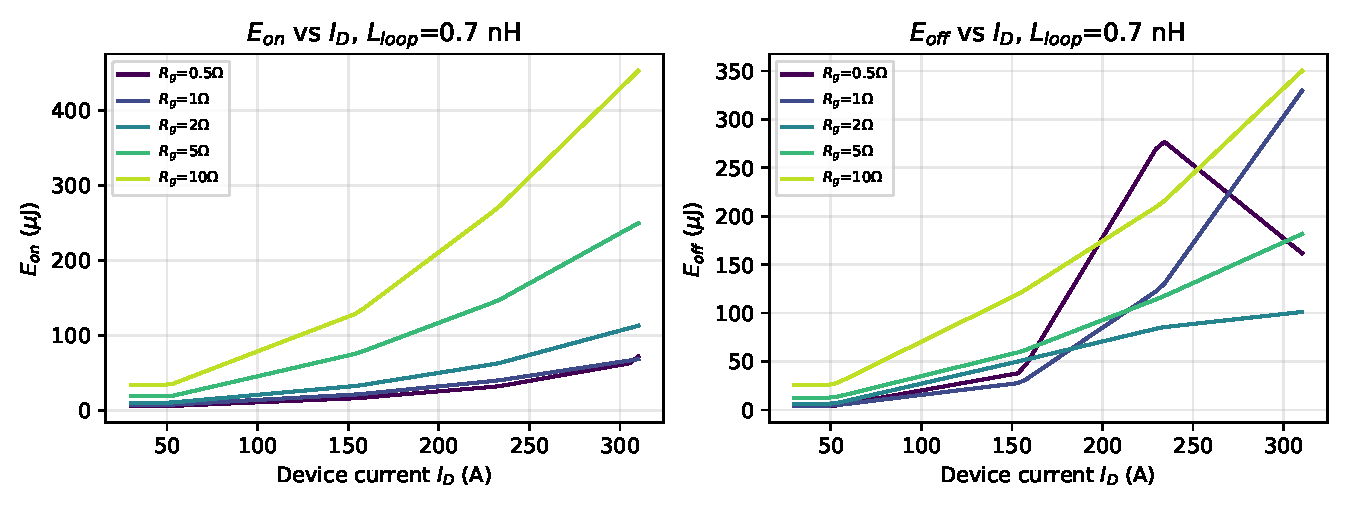
\includegraphics[width=\linewidth]{figures/fig_eon_eoff_vs_rg.pdf}
\caption{$E_{on}$, $E_{off}$ vs.\ device current for $R_g\in\{0.5,1,2,5,10\}\,\Omega$ at
$L_{loop}$=0.7\,nH (LTSpice double-pulse data, EPC2361).}
\label{fig:eon_eoff_rg}
\end{figure}

\begin{figure}[t]
\centering
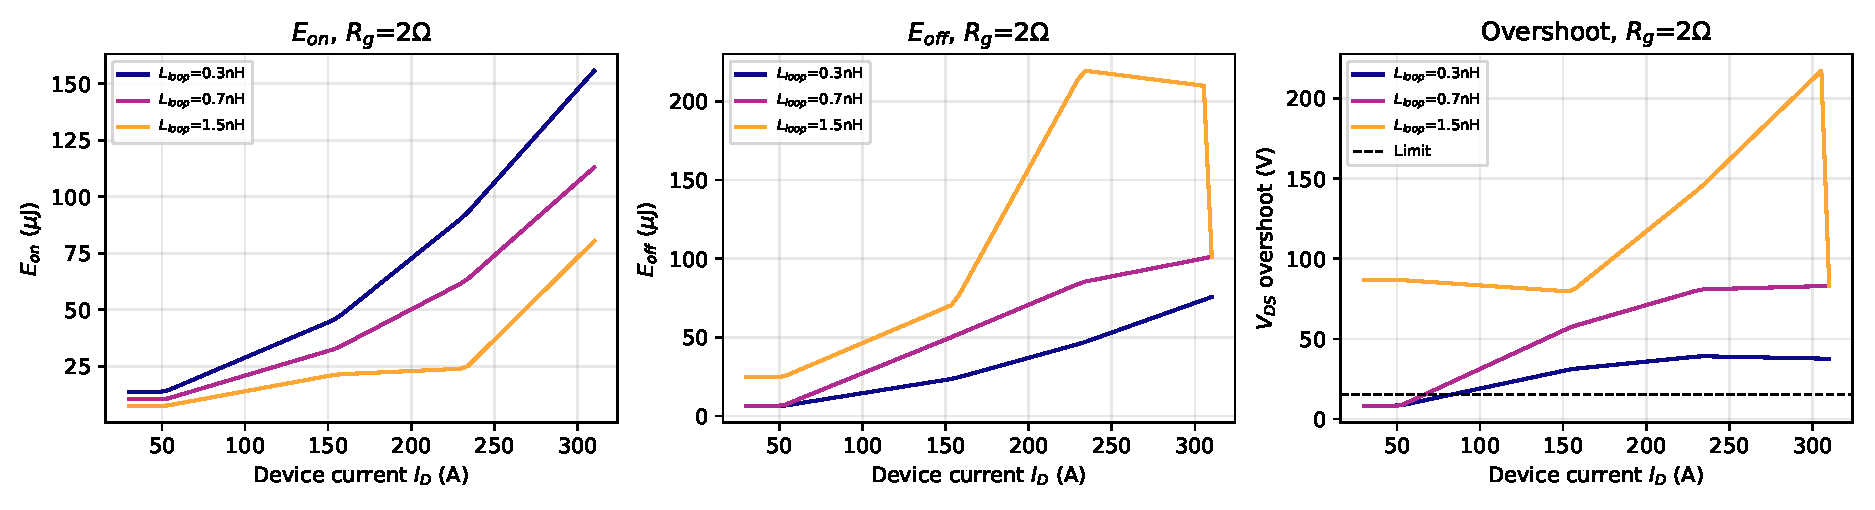
\includegraphics[width=\linewidth]{figures/fig_eon_eoff_vs_lloop.pdf}
\caption{$E_{on}$, $E_{off}$, and $V_{DS}$ overshoot vs.\ device current for
$L_{loop}\in\{0.3,0.7,1.5\}$\,nH at the 2\,\ohm{} reference gate resistance.}
\label{fig:eon_eoff_lloop}
\end{figure}

Figures~\ref{fig:eon_eoff_rg}--\ref{fig:eon_eoff_lloop} show the full characterization:
both $E_{on}$ and $E_{off}$ increase monotonically with device current and gate
resistance at every loop inductance tested (the expected switching-speed/loss
trade-off), while $V_{DS}$ overshoot decreases with $R_g$ and increases sharply with
$L_{loop}$ -- at the largest tested loop inductance (1.5\,nH) and lowest gate
resistances, overshoot exceeds the device's rated $V_{DS,tr}$ margin at high current,
directly motivating a low-inductance layout rather than compensating for a poor one with
gate resistance alone.

\begin{figure}[t]
\centering
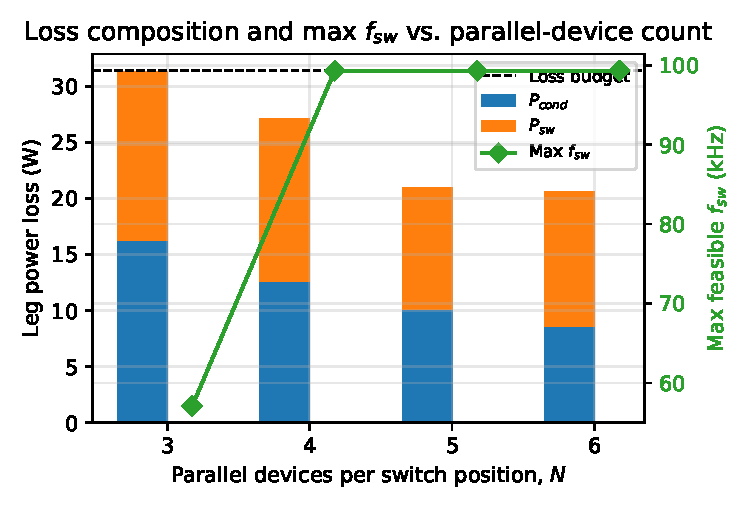
\includegraphics[width=\linewidth]{figures/fig_loss_vs_n.pdf}
\caption{Loss composition and maximum feasible $f_{sw}$ vs.\ parallel-device count $N$.}
\label{fig:loss_vs_n}
\end{figure}

\begin{figure}[t]
\centering
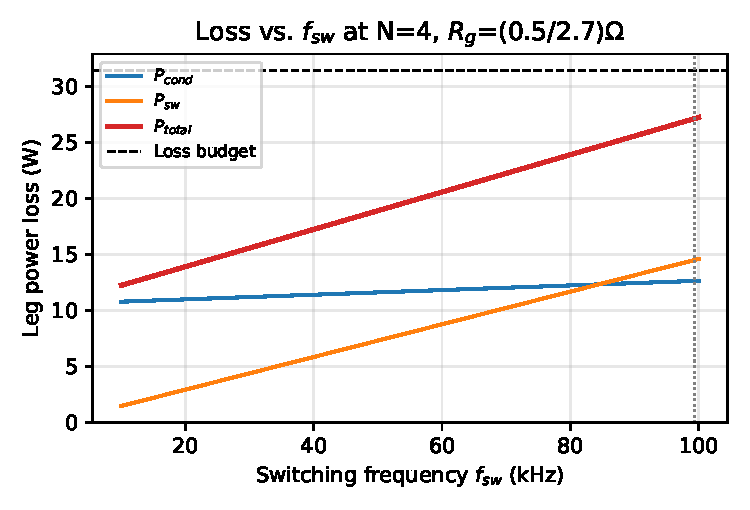
\includegraphics[width=\linewidth]{figures/fig_loss_vs_fsw.pdf}
\caption{Loss vs.\ switching frequency at the recommended design point.}
\label{fig:loss_vs_fsw}
\end{figure}

Figure~\ref{fig:loss_vs_n} sweeps parallel-device count $N$; for each $N$, $R_{g,off}$ is
re-optimized against the overshoot limit and $f_{sw}$ against the loss/thermal budget.
Table~\ref{tab:tradeoff} gives the numeric trade-off. Figure~\ref{fig:loss_vs_fsw} shows
loss composition vs.\ $f_{sw}$ at the recommended point, confirming the search-bound
ceiling discussed below.

\begin{table}[t]
\centering\footnotesize
\caption{$f_{sw}$ vs.\ parallel-device-count trade-off at $L_{loop}$=0.7\,nH (feasible points only).}
\label{tab:tradeoff}
\begin{tabular}{@{}rrrrrrrr@{}}
\toprule
$N$ & $R_{g,on}$ & $R_{g,off}$ & $f_{sw}$ & $P_{total}$ & $T_J$ & Margin & Ovs. \\
 & (\ohm) & (\ohm) & (kHz) & (W) & (\degC) & (\degC) & (V) \\
\midrule
3 & 0.5 & 6.9 & 57.1 & 31.32 & 68.7 & 56.3 & 14.8 \\
\textbf{4} & \textbf{0.5} & \textbf{2.7} & \textbf{99.3} & \textbf{27.12} & \textbf{62.4} & \textbf{62.6} & \textbf{14.8} \\
5 & 0.5 & 0.6 & 99.3 & 20.97 & 57.0 & 68.0 & 14.7 \\
6 & 0.5 & 0.6 & 99.3 & 20.60 & 55.9 & 69.1 & 8.5 \\
\bottomrule
\end{tabular}
\end{table}

\subsection{Recommended design point}

\textbf{N=\NVAL{}, $R_{g,on}$=\RGONVAL\,\ohm, $R_{g,off}$=\RGOFFVAL\,\ohm,
$f_{sw}\approx$\FSWVAL\,kHz}: loss \PTOTALVAL\,W of \PBUDGETVAL\,W budget
(\PCTVAL\% used), $T_J$=\TJVAL\,\degC{} (\MARGINVAL\,\degC{} margin to the 125\,\degC{}
ceiling), $V_{DS}$ overshoot \OVSVAL\,V.

$N$=1 and $N$=2 are infeasible: even at the maximum searched $R_{g,off}$, overshoot
exceeds the 15\,V limit at their per-device currents -- a conclusion from real
double-pulse data, not a rule of thumb. Where the recommended $f_{sw}$ sits at (or near)
the search's configured ceiling with unused loss/thermal margin, that is a
search-bound limit, not a physical one -- raising \texttt{fsw\_max\_Hz} and re-running
would find the true maximum.

%=====================================================================
\section{Discussion and Limitations}
%=====================================================================

\begin{itemize}[leftmargin=1.2em,itemsep=1pt]
\item \textbf{Even current sharing across $N$ parallel devices is assumed}, not modeled.
  Palma et al.~\cite{palma2024} show real boards see dynamic imbalance from
  device-to-device $V_{th}$ spread; layout symmetry (e.g.\ the ``butterfly'' gate-loop
  structure of Wattenberg et al.~\cite{wattenberg2023}, achieving $<$17\% gate-loop
  impedance spread across 8 parallel devices) is essential and not something this model
  can check.
\item \textbf{Steady-state, full-load thermal only} -- no transient/duty-cycled $T_J$
  model (the FEA Foster ladder is recorded in \texttt{data/devices/EPC2361.yaml} for
  future extension).
\item \textbf{Loop inductance} is bounded, not pinned to a single assumed value, by
  sweeping $L_{loop}$ -- but all three values are analytical/literature estimates until
  measured on real hardware.
\item \textbf{Crosstalk/false-turn-on} is not modeled; $R_{g,on}$ is chosen purely to
  minimize switching loss, which may be more aggressive than a real gate-driver's
  pull-down strength and PCB layout can safely support (\S\ref{sec:thermal}).
\end{itemize}

%=====================================================================
\begin{thebibliography}{9}\footnotesize
\bibitem{epc2361} EPC2361 datasheet, rev.\,2.4, Efficient Power Conversion Corp., 2026.
\bibitem{epc2361therm} EPC2361 Thermal SPICE Model, Efficient Power Conversion Corp.
\bibitem{cooke2025} M.\,W.\,J.\ Cooke, D.\,J.\ Rogers, ``120\,V, 155\,A Traction Inverter
  Using Eight Parallel GaN HEMTs,'' 2025/2026.
\bibitem{brothers2019} J.\,A.\ Brothers, T.\ Beechner, ``GaN Module Design
  Recommendations Based on the Analysis of a Commercial 3-Phase GaN Module,'' IEEE ECCE,
  2019.
\bibitem{palma2024} M.\ Palma, V.\ Barba, S.\ Musumeci, ``Parallel Connection of GaN
  FETs: an Experimental Investigation Approach,'' PCIM Europe, 2024.
\bibitem{wattenberg2023} M.\ Wattenberg, O.\,G.\ Lorenz, J.\ Sanchez, ``A Multi-Kilowatt
  Low-Profile GaN Inverter for Light Electric Vehicles and High-Power Tools,'' IEEE APEC,
  2023.
\bibitem{casanellas1994} F.\ Casanellas, ``Losses in PWM inverters using IGBTs,'' IEE
  Proc.\ Electr.\ Power Appl., 1994.
\end{thebibliography}

\end{document}
